% -----------------------------------------------------------------
% Desenvolvido por Filipe Fernandes para o LIPES (Laboratório de Inovação, Pesquisa e Engenharia de Software)
% filipe.fernandes@ifsudestemg.edu.br
% ----------------------------------------------------------------
% Adaptado de Template Latex - Apresentação - UFMG
% https://www.overleaf.com/latex/templates/template-latex-apresentacao-ufmg/ygvvbrrsqgkv
% -----------------------------------------------------------------
% Licença Creative Commons CC BY 4.0
% -----------------------------------------------------------------
% PARA CORRER pdflatex -shell-escape main.tex
\documentclass[aspectratio=169,english]{beamer}

% a opção hideSubsectionTitle esconde o título das subseções
\usepackage{templateLIPES}      % o arquivo templateLIPES.sty possui todo o estilo de formatação
\usepackage[spanish]{babel}     % mude o idioma, caso necessite
\usepackage[alf, abnt-emphasize=bf, abnt-etal-text=it]{abntex2cite}

\setbeamertemplate{bibliography item}{}
\renewcommand{\theenumiv}{}

\begin{document}

\titulo{Incorporación de técnicas de muestreo mediante histogramas multidimensionales al código de
simulación de fuentes de Monte Carlo KDSource}
% \subtitulo{Subtítulo}       % caso não haja, comente

\autor{Lucas Ezequiel Ovando}
\orientador{Dr. Ariel Marquez}        % caso não haja, comente
\coorientador{Ing. Zoe Prieto}      % caso não haja, comente

\juradoA{Dr. Edmundo Lopasso}
\juradoB{Mg. Norberto Schmidt}

\curso{Ingenieria Nuclear}

\local{San Carlos de Bariloche, Rio Negro, Argentina}
\dia{19}
\mes{febrero}
\ano{2025}

% NÃO REMOVA!
\begin{frame}[plain]
    
    \begin{tikzpicture}[overlay,remember picture]
        \node[left=-0.15cm] at (current page.0){
            
\includegraphics[scale=0.145]{imagens/capaLIPES}
        };
    \end{tikzpicture}

    \titlepage
    
\end{frame}

\section[Resumen]{}

\begin{frame}[allowframebreaks]
    \frametitle{Resumen}
    \tableofcontents
\end{frame}

% CONTEÚDO -----------------------------------------------------------------

\section{Motivación}
\begin{frame}{Motivación}
    \begin{itemize}[itemsep=1.5em]
        \item \textbf{Problema:} En cálculos Monte Carlo de blindaje y extracción de haces de neutrones, se necesita determinar el flujo de radiación a grandes distancias de la fuente, en zonas de bajo flujo.
        % \item \textbf{Desafío:} El cálculo de blindajes implica evaluar flujos en regiones con niveles muy bajos, lo que complica la simulación.
        \item \textbf{Solución:} Reducir tiempos de cómputo mediante técnicas de reducción de varianza.
        \item \textbf{Enfoque:} Incorporar técnicas de muestreo con histogramas multidimensionales en el código de simulación Monte Carlo KDSource.
    \end{itemize}
\end{frame}


\section{Introdución}
\begin{frame}{Introdución}
    En este trabajo se planea incorporar una:
    \begin{itemize}[itemsep=1.5em]
        \item Tecnica de muestreo...
        \item ... mediante histogramas multidimensionales...
        \item ... al codigo de simulacion de fuentes Monte Carlo KDSource.
    \end{itemize}
\end{frame}

\begin{frame}{Introdución: Tecnica de muestreo}
    \begin{figure}
        \centering
        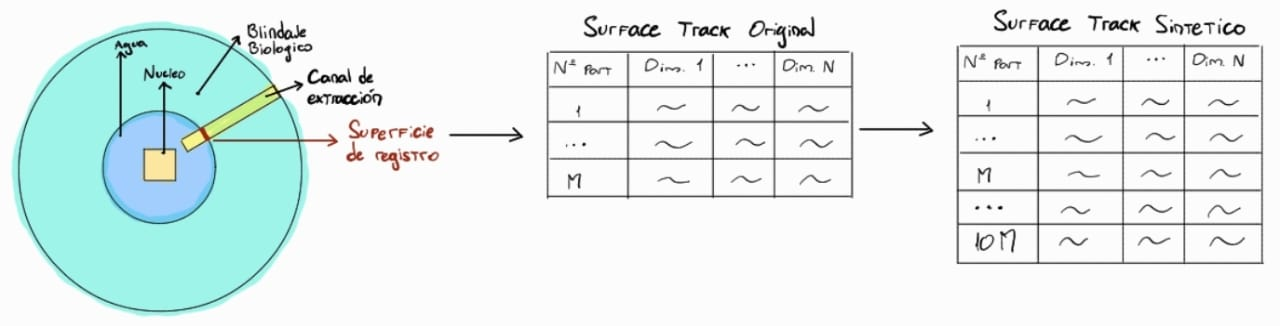
\includegraphics[width=0.95\linewidth]{imagens/esquema1.jpeg}
        % \caption{1º seminário do LIPES em 27/01/2025}
        \label{fig:esquema1}
    \end{figure}

    A partir de una simulacion Monte Carlo se obtiene una lista de las particulas que atraviesan una superficie de registro.\\
    \newline
    Luego se genera una lista de particulas de mayor tamaño para continuar la simulacion desde esa superficie en adelante.
\end{frame}

\begin{frame}{Introdución: Histogramas multidimensionales}
    \begin{figure}
        \centering
        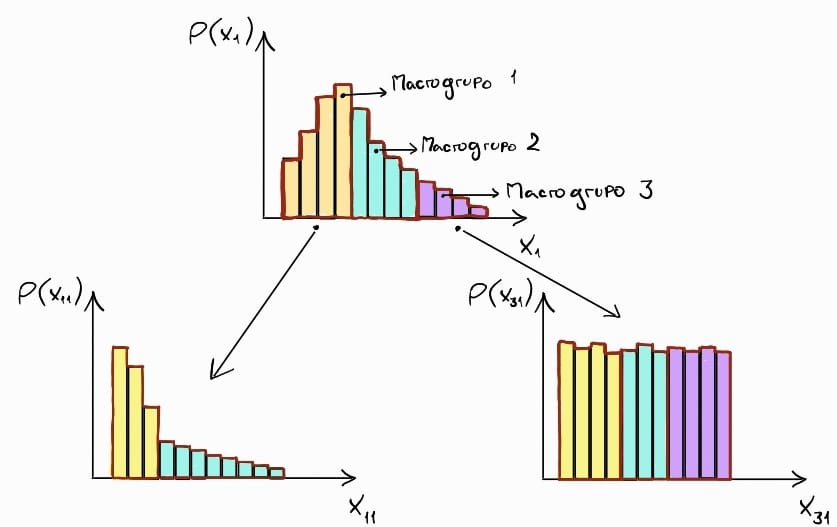
\includegraphics[width=0.35\linewidth]{imagens/esquema2.jpeg}
        % \caption{1º seminário do LIPES em 27/01/2025}
        \label{fig:esquema2}
    \end{figure}

    Se realiza un histograma de la primer variable y se la subdivide en macro grupos. \\
    Luego se realiza subsiguientes histogramas de la siguiente variable para cada macro grupo. \\
    Se repite el proceso hasta formar un arbol de histogramas multidimensionales.\\
    \newline
    Esto se realiza para poder obtener aproximaciones de la distribucion de probabilidad de las variables de interes conservando la correlacion entre las variables.
\end{frame}

\begin{frame}{Introdución: Codigos Monte Carlo: OpenMC y KDSource}
    \begin{figure}
        \centering
        \begin{minipage}{0.35\textwidth}
            \centering
            
\includegraphics[width=\linewidth]{imagens/openmc.png}
            % \caption{Esquema 3}
            \label{fig:openmc}
        \end{minipage}\hfill
        \begin{minipage}{0.35\textwidth}
            \centering
            
\includegraphics[width=\linewidth]{imagens/esquema3.png}
            % \caption{Otra imagen}
            \label{fig:esquema3}
        \end{minipage}
    \end{figure}

    \begin{columns}[t]
        \column{0.45\textwidth}
            \begin{itemize}
                \item Código Monte Carlo open source.
                \item Diseñado para simulaciones de transporte de partículas.
            \end{itemize}
        \column{0.45\textwidth}
            \begin{itemize}
                \item Inicialmente para simular fuentes de neutrones y fotones mediante \textit{kernel density estimation}.
                \item En desarrollo para incorporar histogramas multidimensionales.
                \item Originado en la tesis de maestría de Inti Osiris Abbate.
            \end{itemize}
    \end{columns}
\end{frame}

\section{Resultados preliminares}
\begin{frame}{Resultados preliminares}
    \begin{itemize}
        \item Interiorización del problema y de las tecnicas a incorporar.
        \item Metodo para la aproximación de la distribucion de probabilidad de las variables de interes a traves de histogramas multidimensionales en Python. \textcolor{red}{Por el momento requiere del usuario para la seleccion de parametros y funciona por fuera del codigo de KDSource.}
        \item Metodo para la generación de listas de particulas sinteticas a partir de los histogramas multidimensionales en Python. \textcolor{red}{Por el momento falta traducirlo a C para incorporarlo al codigo de KDSource.}
        \item Resultados preliminares en un canal de extraccion de neutrones.
        \item Todo el trabajo se ha realizado para neutrones, excluyendo los fotones.
    \end{itemize}
    % \begin{figure}
    %     \centering
    %     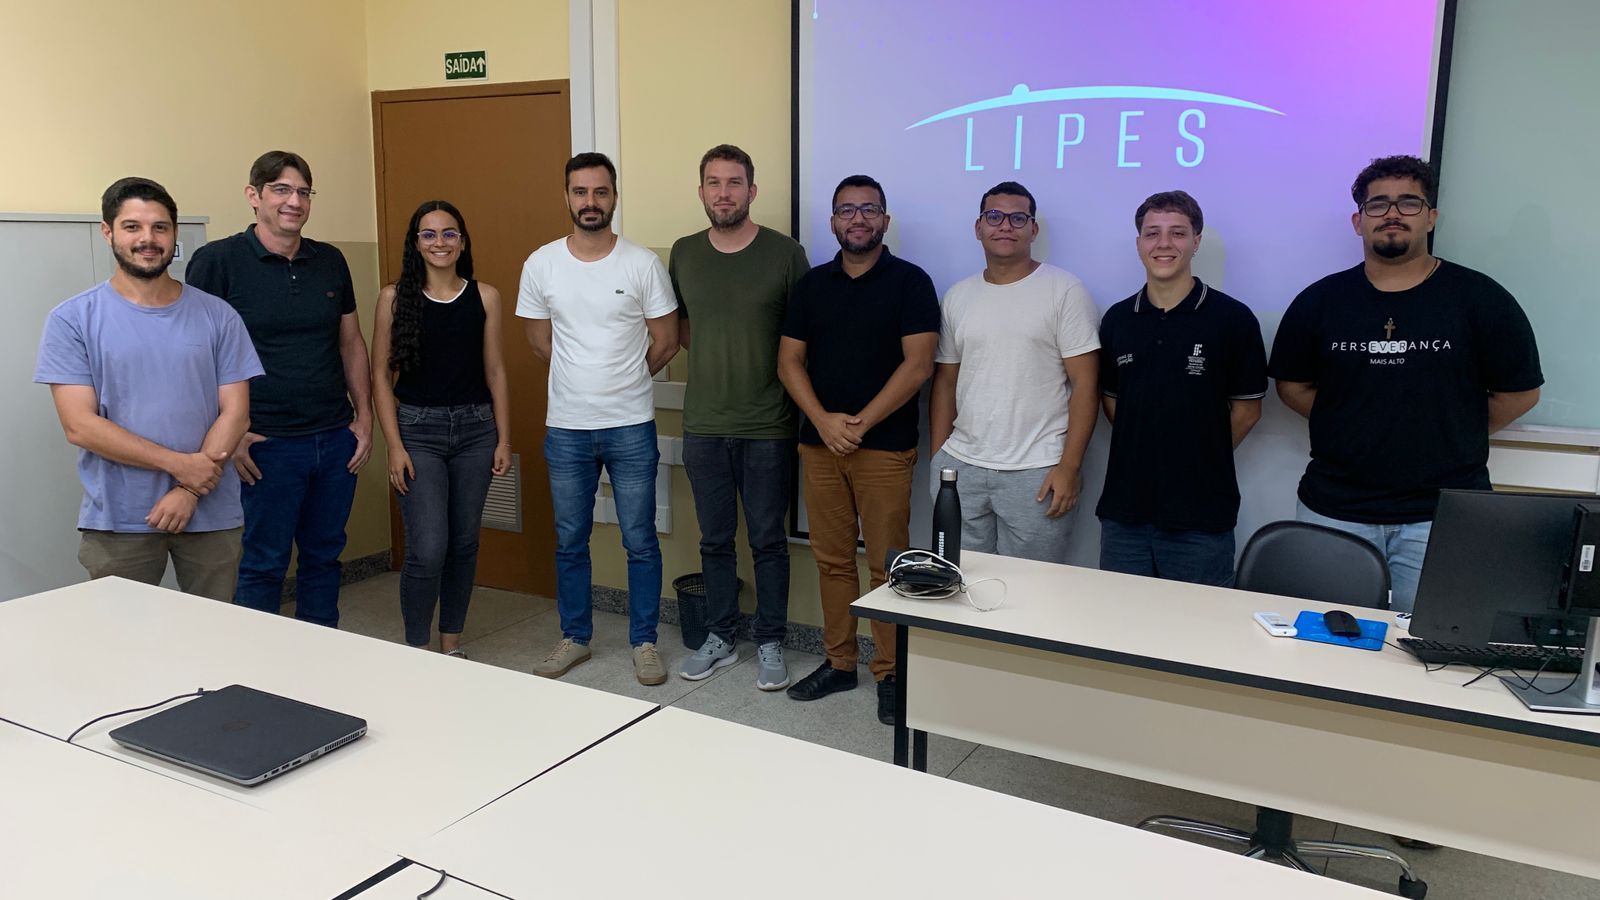
\includegraphics[width=0.6\linewidth]{imagens/1_seminario_LIPES.jpeg}
    %     % \caption{1º seminário do LIPES em 27/01/2025}
    %     \label{fig:1semlipes}
    % \end{figure}

\end{frame}

\begin{frame}[fragile]{Resultados preliminares: Histogramas multidimensionales}
    \textbf{Histogramas macro:}
    \begin{itemize}
        \item Permiten agrupar particulas segun su similutud por variables.
        \item En caso de tomar menos macrogrupos se obtiene mayor estadistica, a costa de perder correlacion entre variables.
        \item El usuario debe seleccionar la cantidad de macrogrupos, el orden del tratamiento de las variables y, de forma opcional, limites de macrogrupos manuales. \textcolor{red}{Por ejemplo, limites geometricos del canal de extracción.}
    \end{itemize} 

    Input tipico:

    \begin{minted}[frame=single, linenos=false]{python}
    orden_columnas = ['letargia', 'x', 'y', 'mu', 'phi']
    macro_grupos = [6,5,5,4]
    \end{minted}

\end{frame}

\begin{frame}[fragile]{Resultados preliminares: Histogramas multidimensionales}
    % Explicacion de un input tipico:

    \begin{minted}[frame=single, linenos=false]{python}
    orden_columnas = ['letargia', 'x', 'y', 'mu', 'phi']
    macro_grupos = [6,5,5,4]
    \end{minted}

    \begin{figure}
        \centering
        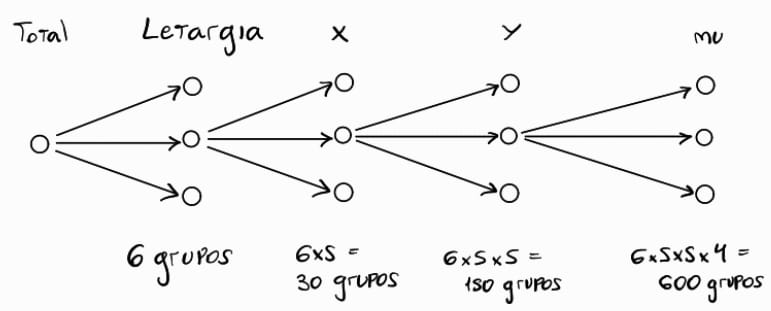
\includegraphics[width=0.7\linewidth]{imagens/esquema3.jpeg}
        % \caption{Total: 1 + 30 + 150 + 600 = 781 grupos macro en estructura de arbol.}
        \label{fig:esquema31}
    \end{figure}

    \begin{itemize}
        % \item Se obtiene un histograma macro de 6 grupos de letargia
        % \item Luego se obtienen un histograma macro de 5 grupos de x para cada grupo en letargia. \\En total 30 grupos de x.
        % \item Luego se obtienen un histograma macro de 5 grupos de y para cada grupo en x. \\En total 150 grupos de y.
        % \item Luego se obtienen un histograma macro de 4 grupos de mu para cada grupo en y. \\En total 600 grupos de mu.
        \item Total: 6 + 30 + 150 + 600 = 786 grupos macro en estructura de arbol.
    \end{itemize}
    % \newline
    \textcolor{red}{Luego, para cada grupo macro se obtiene un histograma micro de la variable de interes.}

\end{frame}

\begin{frame}[fragile]{Resultados preliminares: Histogramas multidimensionales}
    \textbf{Histogramas micro:}

    \begin{figure}
        \centering
        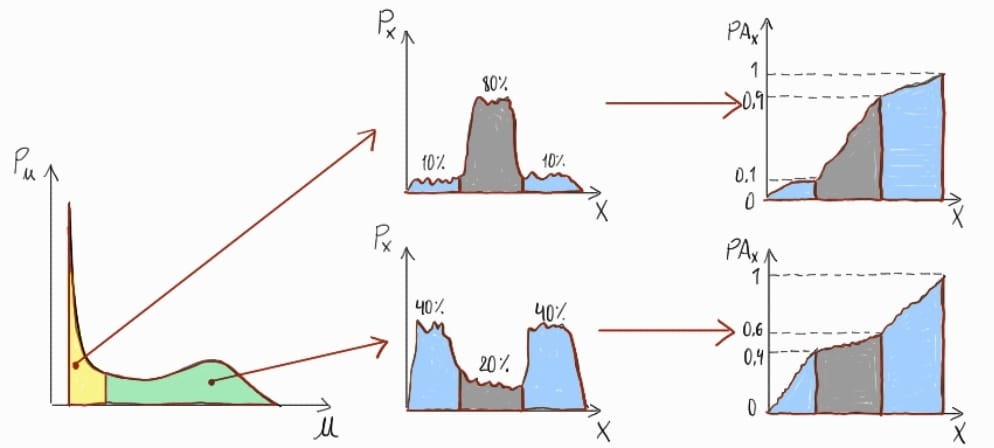
\includegraphics[width=0.55\linewidth]{imagens/esquema4.jpeg}
        % \caption{Total: 1 + 30 + 150 + 600 = 781 grupos macro en estructura de arbol.}
        \label{fig:esquema4}
    \end{figure}

    \begin{itemize}
        % \item Para cada macro grupo se obtiene un histograma micro de la variable de interes.
        % \item A partir del histograma se normaliza y se obtiene la distribucion de frecuencia acumulada.
        \item La elección del numero de microgrupos es un compromiso entre obtener una buena aproximación de la distribución de probabilidad y evitar reproducir el ruido estadistico.
        \item A partir de este enfoque de macro y micro histogramas se logra aproximar la correlación intrinseca entre las variables de interes.
    \end{itemize}


    \textcolor{red}{Luego es posible muestrear listas de particulas sinteticas a partir de los histogramas multidimensionales, utilizando numeros pseudoaleatorios y las funciones de frecuencia acumulada.}

    % BORRADOR: tal vez poner dos esquemas de muchos y pocos micro bines. Sino ver que hacer para que no quede tan vacia
     

\end{frame}

\begin{frame}{Resultados preliminares: Muestreo de particulas}
    \begin{figure}
        \centering
        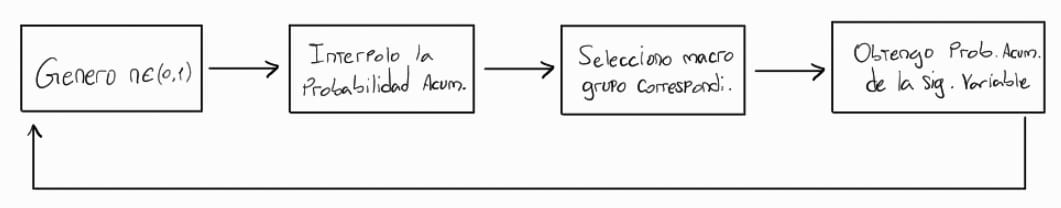
\includegraphics[width=0.95\linewidth]{imagens/esquema5.jpeg}
        % \caption{Total: 1 + 30 + 150 + 600 = 781 grupos macro en estructura de arbol.}
        \label{fig:esquema5}
    \end{figure}

    \begin{itemize}
        % \item Para cada variable se genera un numero pseudoaleatorio entre 0 y 1 y se interpola la inversa de la funcion de frecuencia acumulada para obtener el valor de la variable. 
        % \item Una vez obtenido el valor de la variable, se selecciona el macro grupo correspondiente y se obtiene la funcion de frecuencia acumulada correspondiente para la siguiente variable.
        % \item Se repite el proceso hasta obtener todas las variables de interes.
        \item Se generan N particulas sinteticas y se exportan con formato .h5 para poder ser leidas como fuente por OpenMC.
        \item Se contrasta el resultado de la simulacion de la lista de particulas original y la lista de particulas sinteticas.
    \end{itemize}

\end{frame}

\begin{frame}{Resultados preliminares: Ejemplo de aplicacion}
    % \begin{figure}
    %     \centering
    %     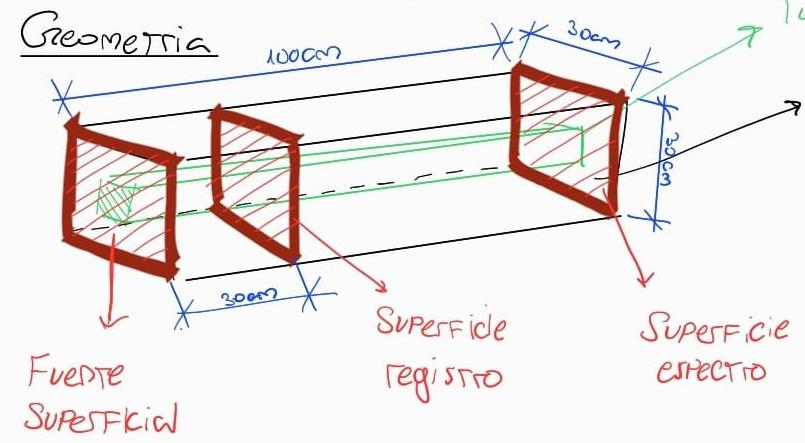
\includegraphics[width=0.55\linewidth]{imagens/croquis1.jpeg}
    %     % \caption{Total: 1 + 30 + 150 + 600 = 781 grupos macro en estructura de arbol.}
    %     \label{fig:croquis1}
    % \end{figure}
    
    % \centering
    % Caracteristicas de la fuente:
    % \begin{itemize}
    %     \centering
    %     \item Monoenergetica de $1 MeV$
    %     \item Uniforme en el plano $XY$
    %     \item Colimada en $\mu = 1$ 
    % \end{itemize}

    \begin{columns}
        \column{0.7\textwidth}
        \begin{figure}
            \centering
            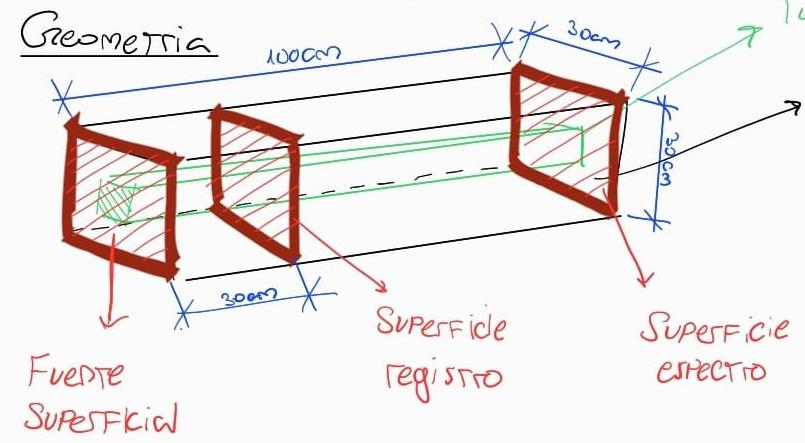
\includegraphics[width=\linewidth]{imagens/croquis1.jpeg}
            \label{fig:croquis1}
        \end{figure}
        
        \column{0.35\textwidth}
        Caracteristicas de la fuente:
        \begin{itemize}
            \item Monoenergetica de $1 \, MeV$
            \item Uniforme en el plano $XY$
            \item Colimada en $\mu = 1$ 
        \end{itemize}
    \end{columns}

\end{frame}

\begin{frame}{Resultados preliminares: Ejemplo de aplicacion}
    \begin{figure}
        \centering
        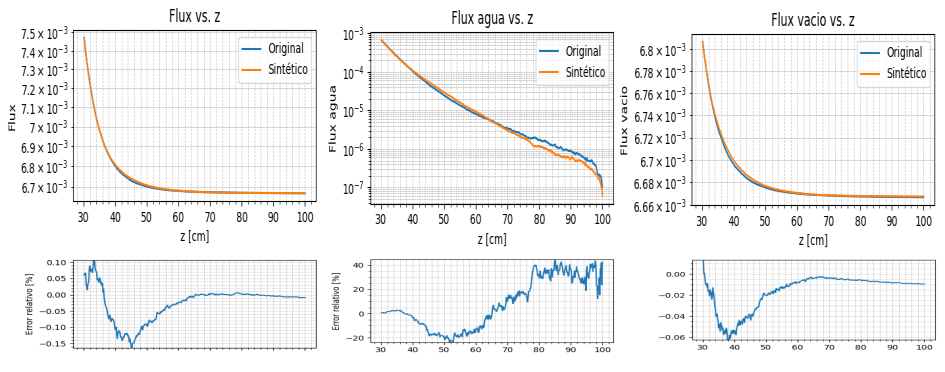
\includegraphics[width=0.9\linewidth]{imagens/flujos.png}
        \label{fig:flujos.png}
    \end{figure}
    \textcolor{red}{Falta poner los datos de esta simulacion. Pero no los puse porque despues voy a hacer estos graficos de vuelta y tal vez uso otros inputs.}
    

\end{frame}

\begin{frame}{Resultados preliminares: Ejemplo de aplicacion}
    
    \textcolor{red}{Aca voy a poner un grafico como el anterior pero del espectro al final del tubo.}
    

\end{frame}

% \begin{frame}{Resultados preliminares: Ejemplo de aplicacion}
%     Entre ellos comentar diferencias entre incorporar o no los limites manuales de los macrogrupos (geometricos y en letargia). \\
%     Ademas comentar diferencias entre diferente cantidad de micro y macrogrupos. Y tambien entre mayor o menor cantidad de particulas registradas.\\
%     Ademas comentar del tubo de vacio y caracteristicas delticas de la fuente que estamos utilizando (delta en mu y en letargia).\\
%     Ademas comentar que miramos el flujo a traves de la dimension de propagacion (total, agua y vacio) y que se observa el espectro al final del tubo (total, agua y vacio).

    

% \end{frame}

\section{Conclusiones preliminares}
\begin{frame}{Conclusiones preliminares}
    \begin{itemize}
        \item Comentar las caracteristicas delticas de la fuente que estamos utilizando (delta en mu y en letargia). Comentar que es relevante porque luego de un colimador el haz es bastante monodireccional.
        \item Hablar sobre la ventaja de utilizar histogramas en vez de gaussianas para seguir este tipo de fenomenos.
        \item Comentar la importacia de seleccionar manualmente los limites de los macrogrupos, tanto los geometricos como los de letargia.
        \item Comentar la importacia de seleccionar una cantidad apropiada de macro y micro bines.
    
    \end{itemize}

\end{frame}

\section{Trabajo futuro}
\begin{frame}{Trabajo futuro}

    \begin{itemize}
        \item Incorporracion de seleccion de parametros automaticos (tal vez decir que lo de la distancia KL).\\
        \item Ver de simular un caso real donde el haz no es 100\% monodireccional sino que tiene algun grado de dispersion.\\
        \item Incorporar a la API de KDSource los metodos de histogramas multidimensionales.\\
        \item Incorporar a la API de KDSource el metodo de muestreo de particulas sinteticas. \textcolor{red}{Esto incluye traducirlo a C y el acople on the fly.}\\
        \item Aplicacion en el conducto N5 del RA6 para la simulacion del CHOPPER. \textcolor{red}{En este ejemplo podemos calcular a traves de la simulacion del RA6 y comparar contra medicion.}\\
    \end{itemize}


\end{frame}

% \section{Código}
% \begin{frame}[fragile]{Código}
% \begin{minted}{python}
% from qiskit import QuantumRegister, QuantumCircuit
% from numpy import pi

% qreg_q = QuantumRegister(2, 'q')
% circuit = QuantumCircuit(qreg_q)

% circuit.h(qreg_q[0])
% circuit.cx(qreg_q[0], qreg_q[1])
% \end{minted}
% \end{frame}

% \section{Citação}
% \begin{frame}{Citação}
%     \begin{itemize}
%         \item De acordo com \citeonline{fernandes2017} ...
%         \item ... lorem ipsum \cite{fernandes2023}.
%     \end{itemize}
% \end{frame}

% FIM DO CONTEÚDO -----------------------------------------------------------------

% NÃO REMOVA! 
% Comentarios: benchmark GODIVA para anexo. 
\section{Referências}
\begin{frame}[allowframebreaks]
    \addtocounter{framenumber}{-1}
    \frametitle{Referências}
    \scriptsize
    % \bibliographystyle{abntex2-alf-en}  % mude para qualquer arquivo .bst
    \bibliography{referencias}
\end{frame}     
\end{document}